\subsection{Glyph: \glyph{Simple chemical}}
\label{sec:simpleChemical}

A simple chemical in SBGN is defined as the opposite of a macromolecule (\sect{macromolecule}): it is a chemical compound that is \emph{not} formed by the covalent linking of pseudo-identical residues. 
Examples  are an atom, a monoatomic ion, a salt, a radical, a solid metal, a crystal, etc.

\begin{glyphDescription}

\glyphSboTerm
SBO:0000247 ! simple chemical


\glyphIncoming
Zero or more \glyph{production} arcs (\sect{production}).



\glyphOutgoing
Zero or more \glyph{consumption} arcs (\sect{consumption}), \glyph{modulation arcs} (\sect{modulations}), \glyph{logic arcs} (\sect{logicArc}), or \glyph{equivalence arcs} (\sect{equivalenceArc}).


\glyphContainer
A \glyph{simple chemical} is represented by a ``stadium'' shape, that is two semicircles of the same radius joined by parallel line segments, as shown in \fig{simpleChemical}.
If desired the parallel line segments can have zero length, and the shape is then identical to a circle.
To avoid confusion with the \glyph{unspecified entity} (\ref{sec:unspecifiedEntity}), this form of the glyph must remain a circle and cannot be deformed into an ellipse.
\glyphLabel
A \glyph{simple chemical} is identified by a label  that is a string of characters that may be distributed on several lines to improve readability.
The centre of the label must be placed on the centre of the container.


\glyphAux
A \glyph{simple chemical} can carry one or more \glyph{units of information} (\sect{unitInfo}).
% These can characterise <EXAMPLES>.
Particular \glyph{units of information} are available for describing the material type (\sect{material-types-cv}) and the conceptual type (\sect{conceptual-types-cv}) of a \glyph{simple chemical}.

A \glyph{simple chemical} can also carry a \glyph{simple clone marker} (see \sect{cloneMarker}).

\end{glyphDescription}

\begin{figure}[H]
  \centering
  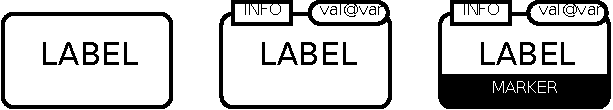
\includegraphics{images/build/simple_chemical_combined.pdf}
  \caption{The \PD glyph for a \glyph{simple chemical}, shown plain and unadorned on the left, with an additional \glyph{unit of information} in the middle, and with a \glyph{simple clone marker} on the right.}
  \label{fig:simpleChemical}
\end{figure}

% The following is for [X]Emacs users.  Please leave in place.
% Local Variables:
% TeX-master: "../sbgn_PD-level1"
% End:
